\documentclass[10pt,a4paper]{article}
\usepackage[utf8]{inputenc}
\usepackage[T1]{fontenc}
\usepackage[margin=1.8cm]{geometry}
\usepackage{lmodern}
\usepackage{microtype}
\usepackage{booktabs}
\usepackage{array}
\usepackage{tabularx}
\usepackage{graphicx}
\usepackage{xcolor}
\usepackage{tikz}
\usepackage{pgfplots}
\usepgfplotslibrary{statistics}
\usepackage{hyperref}
\usepackage{fancyhdr}
\usepackage{float}
\usepackage{enumitem}
\pgfplotsset{compat=1.18}
\definecolor{freecolor}{HTML}{1769AA}
\definecolor{germancolor}{HTML}{D97706}
\definecolor{ink}{HTML}{243447}
\hypersetup{colorlinks=true,linkcolor=freecolor,urlcolor=freecolor}
\pagestyle{fancy}
\fancyhf{}
\lhead{Touring Polygons}
\rhead{Auditoria dos benchmarks}
\cfoot{\thepage}
\setlength{\parindent}{0pt}
\setlength{\parskip}{5pt}
\newcommand{\free}{\textcolor{freecolor}{\textbf{ordem livre}}}
\newcommand{\german}{\textcolor{germancolor}{\textbf{solver alemão}}}
\title{Auditoria e comparação dos benchmarks\\[3pt]\large Touring Polygons}
\author{Relatório reprodutível a partir dos dois CSVs finais}
\date{2026-09-20}
\begin{document}
\maketitle

\begin{abstract}
Este relatório verifica a integridade dos resultados finais e compara o solver de ordem livre com o solver alemão de ordem fixa. A análise usa somente os dois CSVs canônicos, sem recuperar métricas de arquivos intermediários. O resultado principal é uma vantagem consistente do solver de ordem livre: ele certificou todas as 558 instâncias, enquanto o solver alemão certificou 498 das 557 instâncias comparáveis dentro dos limites usados.
\end{abstract}

\section*{Resumo executivo}
\begin{tabularx}{\textwidth}{@{}>{\bfseries}lXXXXX@{}}
\toprule
Solver & Instâncias & Exatas & Taxa exata & Mediana exata (s) & Média exata (s) \\
\midrule
\free & 558 & 558 & 100.0\% & 0.08 & 80.59 \\
\german & 557 & 498 & 89.4\% & 0.31 & 98.84 \\
\bottomrule
\end{tabularx}

No conjunto comum de 557 instâncias exatas para o solver alemão, o speedup definido como $T_{\mathrm{German}}/T_{\mathrm{free}}$ teve mediana 4.47x e média 1 178.15x. Valores acima de 1 favorecem o solver de ordem livre. A comparação deve ser lida como benchmark de engenharia: os solvers têm espaços de busca e métricas internas diferentes.

\section{Verificação dos dados}
\begin{table}[H]
\centering
\caption{Checks automáticos executados sobre os dois arquivos finais.}
\begin{tabularx}{0.95\textwidth}{@{}lXr@{}}
\toprule
Verificação & Critério & Resultado \\
\midrule
Linhas livres & 558 linhas e 558 índices únicos & PASS \\
Linhas alemãs & 557 linhas e 557 índices únicos & PASS \\
Interseção & 557 instâncias comuns, sem duplicações & PASS \\
Exatidão livre & \texttt{exact} coincide com \texttt{termination=optimal} & PASS \\
Exatidão alemã & \texttt{exhausted} e nenhum limite ativo & PASS \\
Branching final & nenhuma linha alemã com \texttt{branch\_limited=true} & PASS \\
Valores não finitos & nenhum token NaN/Inf detectado & PASS \\
\bottomrule
\end{tabularx}
\end{table}

O arquivo alemão exclui a instância 554, que apresentou uma falha determinística \texttt{SIGBUS} no binário alemão. Os hashes SHA-256 dos arquivos analisados estão registrados em \texttt{validation.json}, junto com as contagens completas usadas nesta auditoria.

\section{Instâncias resolvidas ao longo do tempo}
\begin{figure}[H]
\centering
\begin{tikzpicture}
\begin{axis}[
  width=0.94\textwidth, height=7.2cm,
  xmode=log, xmin=0.001, xmax=8000,
  xlabel={Tempo de execução (s, escala logarítmica)},
  ylabel={Instâncias certificadas},
  grid=both, major grid style={gray!22}, minor grid style={gray!10},
  legend style={at={(0.98,0.04)},anchor=south east,draw=none,fill=white},
  every axis plot/.append style={line width=1.2pt},
  tick label style={font=\small}, label style={font=\small}
]
\addplot+[const plot, color=freecolor, mark=none] table [x=time,y=solved] {data/free-ecdf.dat};
\addlegendentry{Ordem livre}
\addplot+[const plot, color=germancolor, mark=none] table [x=time,y=solved] {data/german-ecdf.dat};
\addlegendentry{Solver alemão}
\end{axis}
\end{tikzpicture}
\caption{Número acumulado de instâncias certificadas em função do tempo. A curva alemã termina em 498 porque 59 instâncias atingiram o limite de tempo.}
\end{figure}

\section{Distribuição de tempos e speedup}
\begin{figure}[H]
\centering
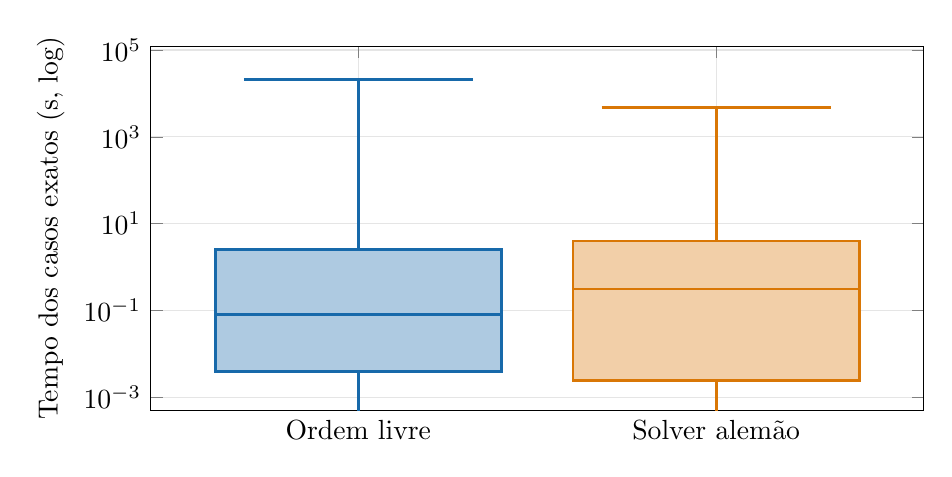
\begin{tikzpicture}
\begin{axis}[
  width=0.94\textwidth, height=6.2cm,
  ymode=log, ymin=0.0005,
  boxplot/draw direction=y,
  xtick={1,2}, xticklabels={Ordem livre,Solver alemão},
  ylabel={Tempo dos casos exatos (s, log)},
  grid=major, major grid style={gray!20},
  every axis plot/.append style={line width=1pt}
]
\addplot+[boxplot prepared={lower whisker=1.2333e-05, lower quartile=0.00381175, median=0.08, upper quartile=2.5603388, upper whisker=20862.6452}, boxplot/draw position=1, fill=freecolor!35, draw=freecolor] coordinates {};
\addplot+[boxplot prepared={lower whisker=8e-06, lower quartile=0.00236725, median=0.31, upper quartile=3.97034075, upper whisker=4787.98947}, boxplot/draw position=2, fill=germancolor!35, draw=germancolor] coordinates {};
\end{axis}
\end{tikzpicture}
\caption{Distribuição dos tempos somente entre instâncias certificadas. O eixo vertical é logarítmico para preservar os casos muito rápidos e os casos difíceis.}
\end{figure}

\begin{figure}[H]
\centering
\begin{tikzpicture}
\begin{axis}[
  width=0.94\textwidth, height=5.8cm,
  xlabel={$\log_{10}(T_{\mathrm{German}}/T_{\mathrm{free}})$},
  ylabel={Número de instâncias},
  ybar, bar width=7pt,
  grid=major, major grid style={gray!20},
  xtick distance=1,
  ymin=0, ymax=73
]
\addplot[fill=freecolor!65, draw=freecolor] table [x=log10_speedup,y=count] {data/speedup-hist.dat};
\addplot[black, dashed, line width=0.8pt] coordinates {(0,0) (0,73)};
\end{axis}
\end{tikzpicture}
\caption{Distribuição do speedup nos 498 casos exatos em ambos os solvers. A linha em zero representa desempenho igual; barras à direita favorecem a ordem livre.}
\end{figure}

\begin{table}[H]
\centering
\caption{Resumo do speedup nos casos exatos comuns.}
\begin{tabular}{@{}lr@{}}
\toprule
Métrica & Valor \\
\midrule
Casos comuns exatos & 498 \\
Mediana & 4.47x \\
Média aritmética & 1 178.15x \\
Percentil 10 / 90 & 0.01x / 352.29x \\
Casos em que ordem livre foi mais rápida & 59.2\% \\
\bottomrule
\end{tabular}
\end{table}

\section{Relação caso a caso}
\begin{figure}[H]
\centering
\begin{tikzpicture}
\begin{axis}[
  width=0.94\textwidth, height=7cm,
  xmode=log, ymode=log,
  xlabel={Tempo da ordem livre (s)}, ylabel={Tempo do solver alemão (s)},
  grid=both, major grid style={gray!22}, minor grid style={gray!10},
  legend style={at={(0.03,0.97)},anchor=north west,draw=none,fill=white},
  tick label style={font=\small}, label style={font=\small}
]
\addplot[only marks, mark=*, mark size=0.8pt, color=freecolor!65, opacity=0.55] table [x=free_seconds,y=german_seconds] {data/runtime-scatter.dat};
\addlegendentry{Casos exatos comuns}
\addplot[dashed, black!65] coordinates {(1.2333e-05,1.2333e-05) (4787.98947,4787.98947)};
\addlegendentry{Mesmo tempo}
\end{axis}
\end{tikzpicture}
\caption{Comparação caso a caso em escala log-log. Pontos acima da diagonal indicam que o solver de ordem livre foi mais rápido.}
\end{figure}

\section{Métricas exclusivas de cada abordagem}

As métricas abaixo não são equivalentes entre si; elas descrevem mecanismos
internos distintos e servem principalmente para diagnosticar por que os custos
de busca diferem.

\begin{table}[H]
\centering
\caption{Métricas internas da ordem livre.}
\begin{tabular}{@{}llrr@{}}
\toprule
Métrica & Coluna & Mediana & P90 \\
\midrule
best updates & \texttt{best\_updates} & 3.00 & 10.00 \\
order space (log2) & \texttt{order\_space\_log2} & 107.71 & 266.23 \\
insertion branches & \texttt{insertion\_branches} & 74.50 & 10 729.00 \\
fallback calls & \texttt{fallback\_calls} & 0 & 468.80 \\
\bottomrule
\end{tabular}
\end{table}

\begin{table}[H]
\centering
\caption{Métricas internas do solver alemão.}
\begin{tabular}{@{}llrr@{}}
\toprule
Métrica & Coluna & Mediana & P90 \\
\midrule
decomposed pieces & \texttt{decomposed\_pieces} & 50.00 & 180.40 \\
grouped pieces & \texttt{grouped\_pieces} & 50.00 & 180.40 \\
best updates & \texttt{best\_updates} & 0 & 1.00 \\
max observed branching & \texttt{max\_observed\_branching} & 5.00 & 9.00 \\
failed prune count & \texttt{failed\_prune\_count} & 60.00 & 14 582.80 \\
\bottomrule
\end{tabular}
\end{table}

\section{Metodologia e limitações}

O solver de ordem livre foi avaliado nas rodadas progressivas de 10, 60, 600 e
3600 segundos; os casos 129 e 541 continuaram em execuções sem limite de tempo
com até um bilhão de chamadas. O solver alemão foi avaliado inicialmente nas
rodadas progressivas até 1800 segundos. Os casos restantes e todos os casos que
tinham sido afetados por limite de branching foram reexecutados por 7200
segundos, com \texttt{max\_branching=-1} e até 100 milhões de chamadas.

As curvas usam o tempo total registrado em \texttt{solver\_seconds}. Para evitar uma
comparação enganosa com execuções interrompidas, os box plots e o speedup usam
somente instâncias certificadas nos dois lados. A curva de instâncias
resolvidas preserva os casos exatos e mostra explicitamente a diferença de
cobertura entre as abordagens.

\end{document}
